\documentclass[12pt,a4paper,table]{article}

\usepackage[a4paper,
            tmargin=2cm,
            bmargin=2cm,
            lmargin=2cm,
            rmargin=2cm,
            bindingoffset=0cm]{geometry}

\usepackage{lmodern}
\usepackage[T1]{polski}
\usepackage[utf8]{inputenc}
\usepackage{tocloft}
\usepackage{hyperref}
\usepackage{amsmath}
\usepackage{listings}
\usepackage{graphicx}
\usepackage{subfig}
\usepackage{float}
\usepackage{booktabs}

\hypersetup{
    colorlinks,
    citecolor=black,
    filecolor=black,
    linkcolor=black,
    urlcolor=black
}


\begin{document}
    \title {
        Teoria współbieżności \\
        Active Object \\
    }

    \author{
        Przemysław Węglik
    }

    \date{\today}

    \maketitle

    \tableofcontents
    \newpage

    \section{Opis Active Object}

    Klienci (obiekty klas $Producent$ i $Consument$) mogą wywoływać metody 
    $pop()$ i $push()$ na obiekcie $Proxy$. 
    Proxy po wywołaniu tych metod, tworzy obiekty żądań.
    Są to obiekty klas $Push$ i $Pop$ dziedziczące po klasie $MethodRequest$.
    Muszą one implementować metody $call()$ oraz $guard()$, które zaimplementowane
    są specyficznie w zależności od rodzaju żądania.

    $Proxy$ zwraca klientom obiekt typu $Promise$ (w innej nomenklaturze $Future$)
    który zawiera informację o tym czy żądanie z nim skojarzone zostało już
    przetowrzone przez serwer (inaczej wszystkie obiekty na procesie serwera:
    $Scheduler$, $Servant$ itp.)

    $Proxy$ po utworzeniu żądań wstawia je do kolejki $Schedulera$.
    $Scheduler$ za pomocą metody dispatch po kolei przetwarza żądania
    biorąc pod uwagę co zwraca metoda $guard()$ żądania, innymi słowy czy można
    to żądanie teraz wykonać.
    W $Schedulerze$ używam $LinkedBlockingQueue$. Jest to blokująca kolejka,
    pozwalająca klientowi, poprzez obiekt $Proxy$, wrzucać requesty.

    Wykonanie żądania polega na wywołaniu metody $call()$ wewnątrz której
    wywoływane są konkretne metody $Servanta$ i dokonywane są operacje 
    na współdzielonej pamięci (w naszym przypadku prostym bufforze zawierającym napisy)

    \section{Opis eksperymentu} 
    \subsection{Metryki i pomiary}
    Jako stałe przyjmujemy:
    \begin{enumerate}
        \item Liczba producentów i konsumentów: $p=k=10$
        \item Czas rzeczywisty działania: $t=10$
        \item Rozmiar buffora: $SIZE=20$
        \item Maksymalny wstawiony element: $MAX\_EL\_SIZE=SIZE/2=10$
    \end{enumerate}

    Zarówno klienci (producenci i konsumenci) jak i serwer (Monitor/Active Object)
    będą wykonywać jakąs dodatkową pracę. W przypadku klienta jest to czas spożytkowany
    na wykonanie dodatkowych zadań. W przypadku serwerra pewien koszt obliczeń.

    Metryką będzie ilość zadań które udało się wykonać klientom dla różnego skomplikowania
    zadania na serwerze. Czyli dla różnego opóźnienia pracy serwera, będziemy obserwować jak radzą sobie 
    z tym klienci.

    Dodatkowa praca jest zaimplementowana w postaci liczenia sinusa z pewnej liczby N razy, 
    gdzie N to $skomplikowanie$ zadania

    Przeprowadzenie pomiarów ograniczyło się do zliczania wykonanych zadań w każdym wątku,
    a potem zliczenia zadań ze wszystkich wątków po ich zakończeniu.
    Każdy pomiar przeprowadzono 10 razy.

    \subsection{Środowisko testowe}
    Testy przeprowadziłem na swoim laptopie Acer Nitro 5 
    z procesorem Intel® Core™ i5-9300H, który posiada 8 rdzeni, 2.4Ghz każdy.
    W trakcie przeprowadzania testów użyłem narzędzia $htop$ do sprawdzenia czy wszystkei rdzenie są używane
    i zgodnie z oczekiwaniami były: 

    \begin{figure}[H]
        \centering
        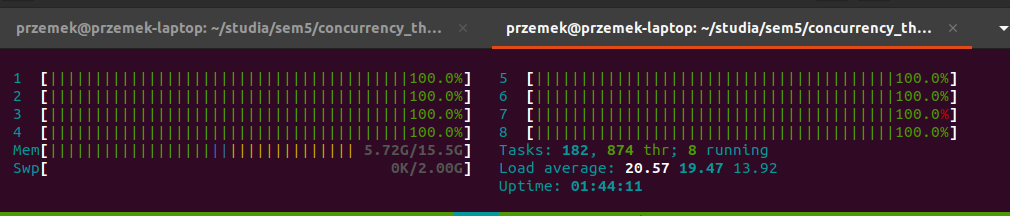
\includegraphics[width=1\linewidth]{img/htop.png}
        \caption{Zrzut ekranu z programu $htop$}
        \label{fig:htop}
    \end{figure}


    \section{Hipoteza}
    Hipoteza jest taka, że w Active Object koszt zadania w serwerze nie 
    powinien mieć wpływu na ilość zadań, ponieważ żądania do serwera wysyłamy asynchronicznie.
    W przypadku działania synchronicznego, ilość zadań powinno spadać wraz z wzrostem
    czasu przetwarzania przez serwer, ponieważ synchronicznie czekamy, aż będzie on znów 
    dostępny.

    Teoretycznie jeśli zadanie wykonywane przez serwer trwa bardzo krótko, to przy dużej liczbie 
    klientów może się okazać, że Monitor będzie szybszy. Obiekty będą przebywały w nim bardzo krótko,
    a nie otrzymujemy dodatkowego obciążenia związanego z utrzymywanie całej architektury AO.


    \section{Wyniki} 
    Pierwszą część hipotezy udało się potwierdzić. Dla stałego kosztu równego $100$ 
    (czyli 100 razy obliczamy sinsua w pętli) w przypadku AO widzimy pewne wahania na wykresie. Są one 
    jednak nieregularne i mogą być związane z różnym obciążeniem komputera przez pozostałe procesy w 
    trakcie wykonywania eksperymentu. W przypadku Monitora widzimy ewidentą tendecję spadkową
    wraz ze wzrostem czasu przetwarzania przez Monitor. Procesy nie są w stanie wykonywać zadań
    czekając na locku Monitora, więc im dłużej muszą czekać, tym tych zadań wykonują mniej. 

    Wart ozauważyć, że nawet w najbardziej korzystnych warunkach wariant synchroniczny wykonuje ponad
    dziesięciokrotnie mniej dodatkowych zadań niż wariant asynchroniczny.

    \begin{figure}[H]
        \centering
        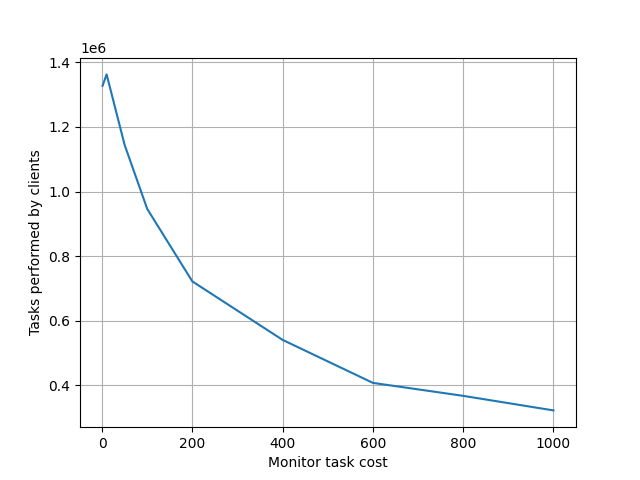
\includegraphics[width=0.8\linewidth]{img/synchro_100client.png}
        \caption{Wykres wykonanynch zadań od kosztu działania Monitora}
        \label{fig:synchro_100client}
    \end{figure}

    \begin{figure}[H]
        \centering
        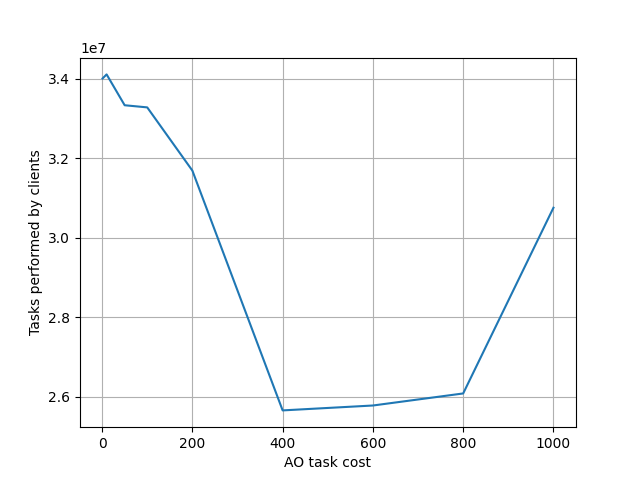
\includegraphics[width=0.8\linewidth]{img/ao_100client.png}
        \caption{Wykres wykonanynch zadań od kosztu działania AO}
        \label{fig:ao_100client}
    \end{figure}


    Co do drugiej części hipotezy nie udało mi się tego dowieźć. Sprawdzałem zarówno bardzo duże (po 200),
    jak i małe (po 2) liczby producentów i konsumentów. Manipulowałem stosunkiem koszt serwera/koszt klienta.
    Za każdym razem okazywało się, że AO był wielokrotnie lepszy. W każdym wypadku może się zdażyć, że
    wątek będzie musiał czekać na Monitor. Na AO nie musimy czekać nigdy i po wrzuceniu zadania w kolejkę,
    możemy oczekiwać na rezultat wykonując dodatkową pracę. Byćmoże wynika to z błędu w implementacji 
    wariantu synchronicznego który spowalnia ją na tyle, że daje niemiarodajne wyniki, lub umieszczenia
    pomiarów w złym miejscu.

    \section{Wnioski}
    Active Object jest dużo efektywniejszym wzorcem w większości standardowych sytuacji.
    Zadania wykonywane przez serwer mogą zająć pewną nieznaną ilość czasu i lepiej tego czasu nie marnować
    na czekanie na odpowiedź.
    Metody synchroniczne przydatne mogą być do bardzo prostych rozwiązań,
    lub jeśli czas zmarnowany na czekanie klientów nie jest problemem.
    Być może na sytuację wpływa ilosć procesów lub sposób implementacji tych wzorców, ale 
    to pozostawiam przyszłym badaczom.


    


\end{document}